\documentclass{article}

\usepackage{fullpage,latexsym,picinpar,amsmath,amsfonts,graphicx, epstopdf } %}
%\epstopdfsetup{update}

\input{macros.tex}

\begin{document}
\centerline{REMOVED}
\centerline{REMOVED}
\centerline{\large \bf CS/MATH111 ASSIGNMENT 5}


\vskip 0.15in

%\noindent{\bf Individual assignment:} Problems 1, 2, and 3.
%\noindent{\bf Group assignment:} Problems 1, 2 and 3.

\vskip 0.15in


%%%%%%%%%%%%%%%%%%%%%%%%%%%%


\begin{problem}
An \emph{edge coloring} of a graph is an
assignment of colors to edges such that any two
edges that share an endpoint have different colors. (It can be proved that if the maximum vertex degree $D \ge 1$, then $G$ can be edge-colored with at most $2D - 1$ colors.)

Here is an example of an edge coloring of
a graph with $5$ colors (colors represented by numbers):

\begin{center}
\includegraphics[width=3.2in]{HW5_pics/graph_edge_color_hw5.pdf}
\end{center}

\noindent
For the graph above, find (show on the graph) an edge coloring with at most $4$ colors.



\end{problem}

\begin{solution}

\begin{center}
\includegraphics[width=3.2in]{HW5_pics/g2.png}
\end{center}

\end{solution}

%%%%%%%%%%%%%%%%%%%%%%%%%%%%

\begin{problem}
Let $G$ and $H$ be the graphs below. For each graph, determine
whether it is bipartite. 
If the graph is bipartite, determine whether it has a perfect matching.
Justify your answer.
%
\begin{center}
{\large Graph $G$:\ }
\begin{minipage}{2in}
        \includegraphics[width=2in]{HW5_pics/graph3_hw5.pdf}
\end{minipage}
\ \ \
{\large Graph $H$:\ }
\begin{minipage}{2.5in}
        \includegraphics[width=2.5in]{HW5_pics/graph4_hw5.pdf}
\end{minipage}
\hfill
\end{center}
\end{problem}


\begin{solution}

\\\\ Graph G is not bipartite, as it can not be separated into either a left or right sorting.
\\\\ The graph has a cycle of odd length: (i, e, f, g, d)
\newline
\\\\ Graph H is bipartite as it has no cycles of odd length and can be broken up into L, R sections:
\\\\ L: B, J, C, I, F
\\\\ R: A, D, H, Y, E
\\\\ This graph also has a perfect match:
\\\\ It has an even number of vertices
\\\\ $|N(x)| >= |X|$ where $|N(x)|$ is the set of neighbors of x.
\\\\ The match can be set as:
\\\\ (B, A), (D, C), (F, E), (J, H), (G, I)

\end{solution}


%%%%%%%%%%%%%%%%%%%%%%%%%%%%
\begin{problem}
Let G be the graph below. 
	\begin{center}
		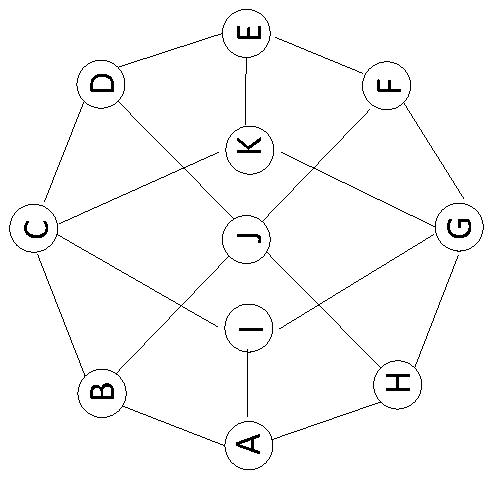
\includegraphics[angle = 270, width = 2in]{HW5_pics/Graph1HW5.eps}
		%\hfill
		%\includegraphics[width = 2.8in]{graphHa_hw5.pdf}
	\end{center}
	
\noindent (a) Determine whether it is bipartite. If the graph is bipartite, determine whether it has a perfect matching. Justify your answer.\\
(b) What is the chromatic number of G? Explain.\\
(c) Does G have a Hamiltonian Path? Justify.\\
(d) Is G a planar graph? (You need to either show a planar embedding or prove, that G is nonplanar.)
\end{problem}

\begin{solution}
\\\\ (a)
\\\\ Graph H is bipartite as it has no cycles of odd length and can be broken up into L, R sections:
\\\\ L: C, A, J, E, G
\\\\ R: B, D, I, K, H, F
\\\\ There is an odd number of vertices here, $|N(x)| >= |X|$ where $|N(x)|$ is the set of neighbors of x is not fulfilled.
\\\\ Therefore there is no perfect matching.
\newline
\\\\ (b) 
\\\\ The chromatic number is 2. This is because this is the minimum amount of colors required so that no two adjacent vertices have the same color.
\newline
\begin{center}
\includegraphics[width=3.2in]{HW5_pics/g7.PNG}
\end{center}
\newline
\\\\
\\\\ (c) G has a Hamiltonian Path: 
\\\\ H,A,I,G,K,C,B,J,F,E,D
\newline
\\\\ (d) G is a planar graph.  This is seen with the planar embedding below:
\begin{center}
\includegraphics[width=3.2in]{HW5_pics/g4.PNG}
\end{center}




\end{solution}

%%%%%%%%%%%%%%%%%%%%%%%%%%%%


\begin{problem}
Determine which of the following two graphs is/are planar/nonplanar.
Justify your answer. (You need to either show a planar embedding or
use Kuratowski's theorem.)

	\begin{center}
		\includegraphics[width = 2.3in]{HW5_pics/graphGa_hw5.pdf}
		\hfill
		\includegraphics[width = 2.8in]{HW5_pics/graphHa_hw5.pdf}
	\end{center}

\end{problem}

\begin{solution}
\\\\ Graph G is non-planar. We use Kuratowski's theorem to find that K, 5 can be found within the graph in the sub graph made up of: (B, E, D, G, C, A)
\newline
\begin{center}
\includegraphics[width=3.2in]{HW5_pics/g5after.PNG}
\end{center}

\newline
\\\\ Graph H is planar.
\begin{center}
\includegraphics[width=3.2in]{HW5_pics/g6.PNG}
\end{center}

\end{solution}
\end{document}

